\chapter*{Plano de Continuidade}

Esta foi a primeira parte do trabalho. Nos meses seguintes, planeja-se: (1) contextualizar e detalhar as ferramentas apresentadas, (2) propor uma combinação dessas ferramentas para o desenvolvimento de aplicações com arquitetura de microsserviços, (3) desenvolver uma aplicação exemplar usando as ferramentas propostas e boas práticas discutidas, (4) analisar pontos positivos e negativos das ferramentas usadas. O cronograma de atividades previstas para serem realizadas na disciplina de Trabalho de Conclusão de Curso 2 é apresentado na \autoref{figura-grafico-gantt}.

\begin{figure}[htb]
	\caption{\label{figura-grafico-gantt}Cronograma de atividades que serão desenvolvidas.}
	\begin{center}
	    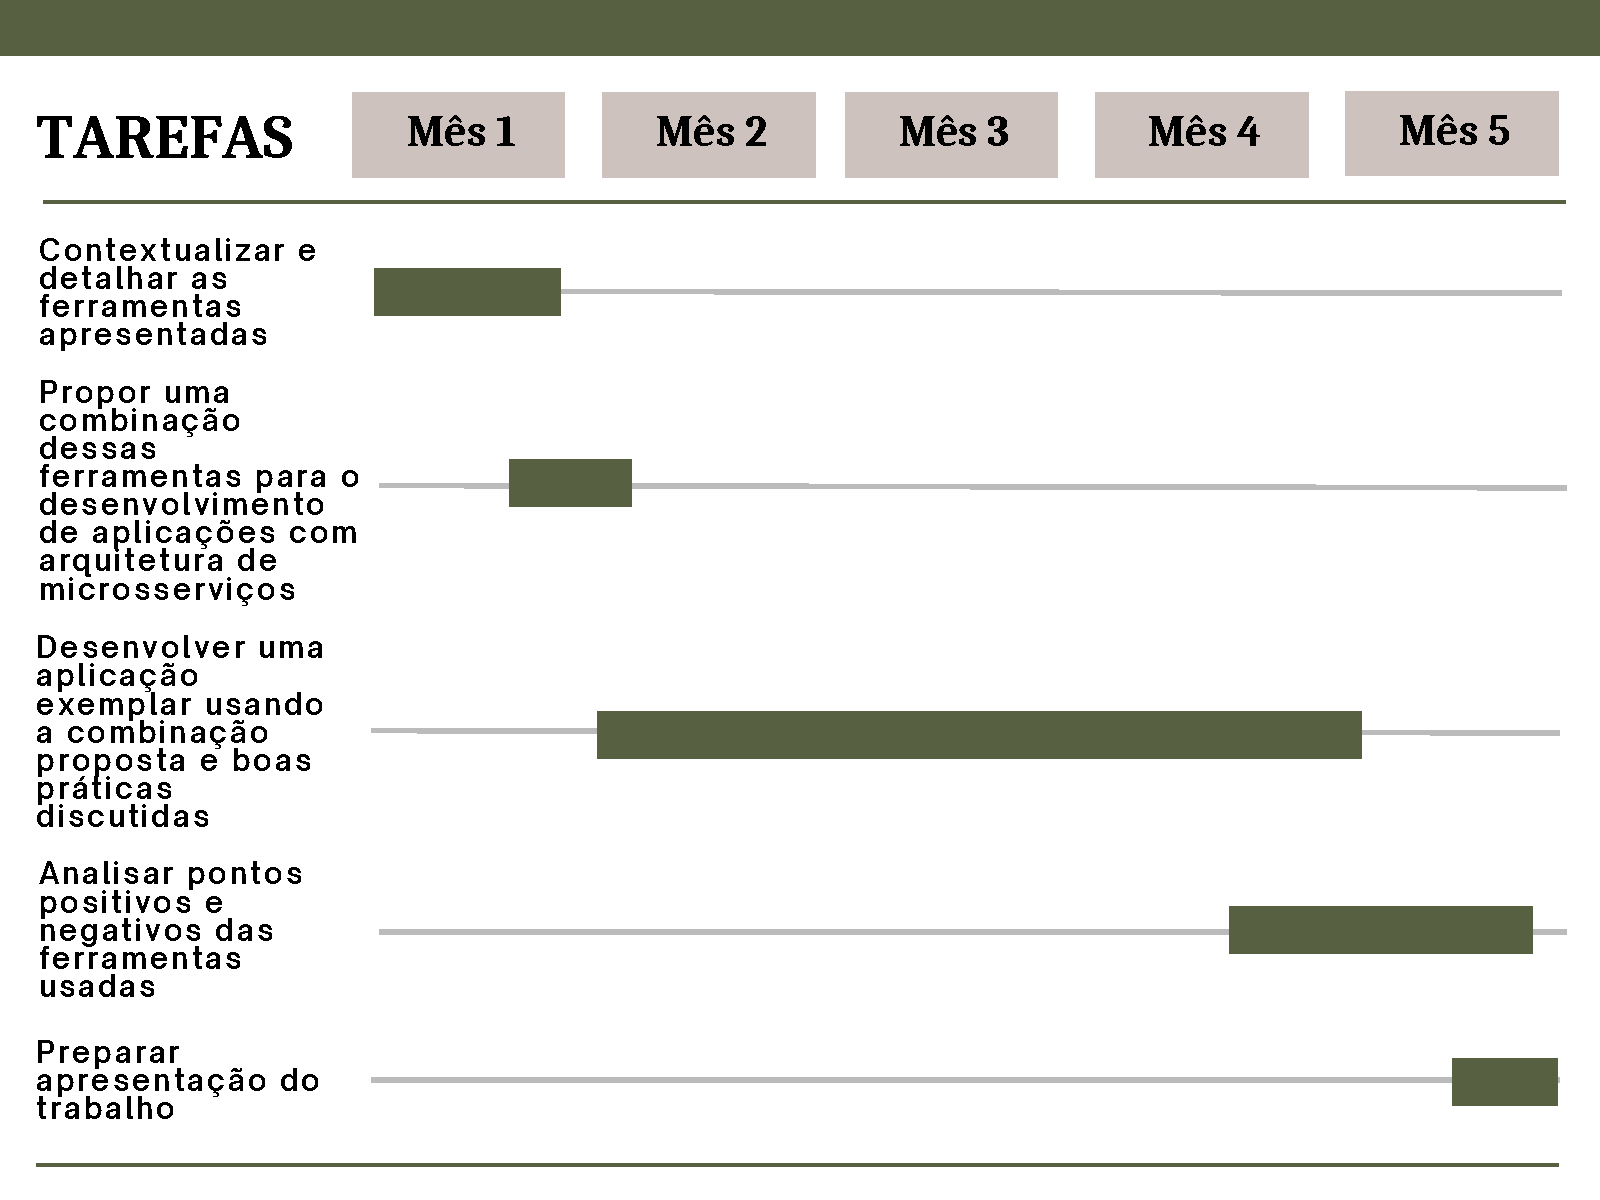
\includegraphics[scale=0.5]{Imagens/grafico-gantt.pdf}
	\end{center}
	\legend{Fonte: Autor}
\end{figure}